\documentclass[10pt]{article}
\usepackage{palatino}
\usepackage{fullpage}
\usepackage{latexsym}
\usepackage{amsfonts}
\usepackage{hyperref}
\usepackage{multicol}
\usepackage{fancyhdr}
\usepackage{enumitem}
\usepackage{caption}
\usepackage{subcaption}
\usepackage{fancybox}
\usepackage{framed}

\pagestyle{empty}                       %no page numbers
\thispagestyle{empty}                   %removes first page number
\setlength{\parindent}{0in}

\usepackage{fullpage}
\usepackage[tmargin = 0.5in, bmargin = 1in, hmargin = 1in]{geometry}     %1-inch margins
\geometry{letterpaper}
\usepackage{graphicx}
\usepackage{amssymb}

	\thispagestyle{empty}
	\renewcommand{\headrulewidth}{0.0pt}
	\thispagestyle{fancy}
	\lhead{Name: \underline{\hspace{1.5in}}}
	\chead{MTH 201: Calculus}
	\rhead{\framebox{\textbf{Grade: \ S \quad P}} }
	\lfoot{}
	\cfoot{}
	\rfoot{}


\begin{document}

	\vspace*{0in}

		\begin{center}
			\textbf{Learning Target C8 \\
			Version 3}
		\end{center}

\emph{Please place all work in the blank below. If you need more room, use the back of this pagee.}

\begin{framed}
	\textbf{C8: Given the graph of a function, identify intervals of increase and decrease, concavity, local extrema, critical points, and inflection points. }
\end{framed}


On the graph of the function below, which is only defined on the interval $[-2,2]$: 

\begin{itemize}
    \item Label the critical numbers. 
    \item Label all local minimums and maximums. (If there are no local extreme values, say so.) 
    \item Label all global minimums and maximums. (If there are no local extreme values, say so.) 
    \item Label all inflection points. 
\end{itemize}
By ``label'', we mean simply indicate these points on the graph (with arrows, circles, etc.). You do not need to give the coordinates as long as the points are clearly indicated, but you do need to say which points are critical numbers, which are inflection points, etc. 

\begin{center}
    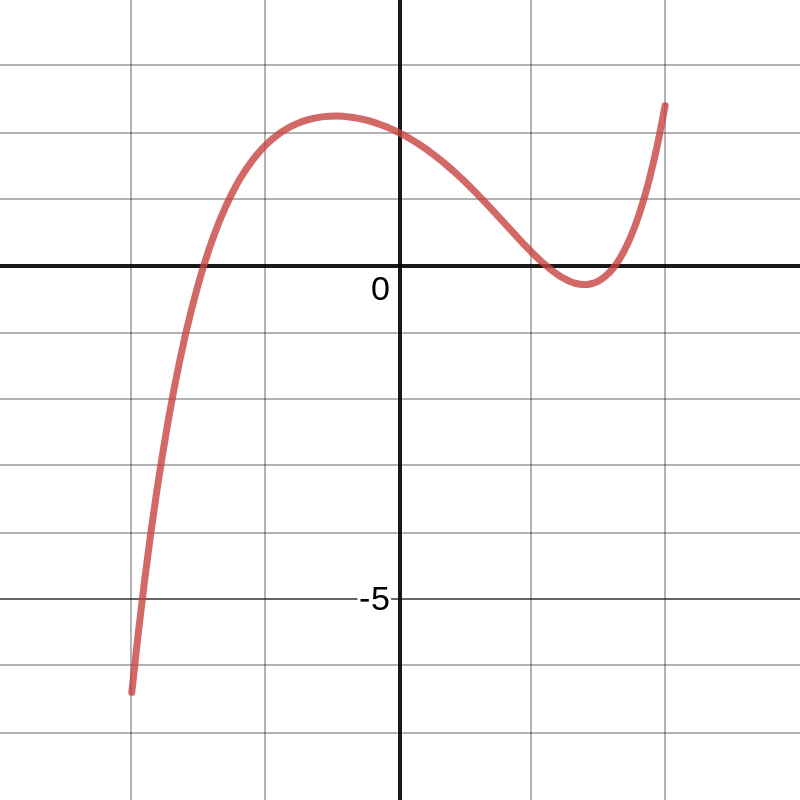
\includegraphics[width=4in]{ltc8-nov14.png}
\end{center}

\vfill

\begin{small}
    \begin{framed}
        	\textbf{Criteria for Satisfactory grade:} All items are correctly labelled with no more than one mistake. 
    \end{framed}

\end{small}

\end{document}
